% Options for packages loaded elsewhere
\PassOptionsToPackage{unicode}{hyperref}
\PassOptionsToPackage{hyphens}{url}
%
\documentclass[
]{book}
\usepackage{amsmath,amssymb}
\usepackage{lmodern}
\usepackage{ifxetex,ifluatex}
\ifnum 0\ifxetex 1\fi\ifluatex 1\fi=0 % if pdftex
  \usepackage[T1]{fontenc}
  \usepackage[utf8]{inputenc}
  \usepackage{textcomp} % provide euro and other symbols
\else % if luatex or xetex
  \usepackage{unicode-math}
  \defaultfontfeatures{Scale=MatchLowercase}
  \defaultfontfeatures[\rmfamily]{Ligatures=TeX,Scale=1}
\fi
% Use upquote if available, for straight quotes in verbatim environments
\IfFileExists{upquote.sty}{\usepackage{upquote}}{}
\IfFileExists{microtype.sty}{% use microtype if available
  \usepackage[]{microtype}
  \UseMicrotypeSet[protrusion]{basicmath} % disable protrusion for tt fonts
}{}
\makeatletter
\@ifundefined{KOMAClassName}{% if non-KOMA class
  \IfFileExists{parskip.sty}{%
    \usepackage{parskip}
  }{% else
    \setlength{\parindent}{0pt}
    \setlength{\parskip}{6pt plus 2pt minus 1pt}}
}{% if KOMA class
  \KOMAoptions{parskip=half}}
\makeatother
\usepackage{xcolor}
\IfFileExists{xurl.sty}{\usepackage{xurl}}{} % add URL line breaks if available
\IfFileExists{bookmark.sty}{\usepackage{bookmark}}{\usepackage{hyperref}}
\hypersetup{
  pdftitle={Mappeeksamen},
  pdfauthor={Håvard C. Lorentzen},
  hidelinks,
  pdfcreator={LaTeX via pandoc}}
\urlstyle{same} % disable monospaced font for URLs
\usepackage{color}
\usepackage{fancyvrb}
\newcommand{\VerbBar}{|}
\newcommand{\VERB}{\Verb[commandchars=\\\{\}]}
\DefineVerbatimEnvironment{Highlighting}{Verbatim}{commandchars=\\\{\}}
% Add ',fontsize=\small' for more characters per line
\usepackage{framed}
\definecolor{shadecolor}{RGB}{248,248,248}
\newenvironment{Shaded}{\begin{snugshade}}{\end{snugshade}}
\newcommand{\AlertTok}[1]{\textcolor[rgb]{0.94,0.16,0.16}{#1}}
\newcommand{\AnnotationTok}[1]{\textcolor[rgb]{0.56,0.35,0.01}{\textbf{\textit{#1}}}}
\newcommand{\AttributeTok}[1]{\textcolor[rgb]{0.77,0.63,0.00}{#1}}
\newcommand{\BaseNTok}[1]{\textcolor[rgb]{0.00,0.00,0.81}{#1}}
\newcommand{\BuiltInTok}[1]{#1}
\newcommand{\CharTok}[1]{\textcolor[rgb]{0.31,0.60,0.02}{#1}}
\newcommand{\CommentTok}[1]{\textcolor[rgb]{0.56,0.35,0.01}{\textit{#1}}}
\newcommand{\CommentVarTok}[1]{\textcolor[rgb]{0.56,0.35,0.01}{\textbf{\textit{#1}}}}
\newcommand{\ConstantTok}[1]{\textcolor[rgb]{0.00,0.00,0.00}{#1}}
\newcommand{\ControlFlowTok}[1]{\textcolor[rgb]{0.13,0.29,0.53}{\textbf{#1}}}
\newcommand{\DataTypeTok}[1]{\textcolor[rgb]{0.13,0.29,0.53}{#1}}
\newcommand{\DecValTok}[1]{\textcolor[rgb]{0.00,0.00,0.81}{#1}}
\newcommand{\DocumentationTok}[1]{\textcolor[rgb]{0.56,0.35,0.01}{\textbf{\textit{#1}}}}
\newcommand{\ErrorTok}[1]{\textcolor[rgb]{0.64,0.00,0.00}{\textbf{#1}}}
\newcommand{\ExtensionTok}[1]{#1}
\newcommand{\FloatTok}[1]{\textcolor[rgb]{0.00,0.00,0.81}{#1}}
\newcommand{\FunctionTok}[1]{\textcolor[rgb]{0.00,0.00,0.00}{#1}}
\newcommand{\ImportTok}[1]{#1}
\newcommand{\InformationTok}[1]{\textcolor[rgb]{0.56,0.35,0.01}{\textbf{\textit{#1}}}}
\newcommand{\KeywordTok}[1]{\textcolor[rgb]{0.13,0.29,0.53}{\textbf{#1}}}
\newcommand{\NormalTok}[1]{#1}
\newcommand{\OperatorTok}[1]{\textcolor[rgb]{0.81,0.36,0.00}{\textbf{#1}}}
\newcommand{\OtherTok}[1]{\textcolor[rgb]{0.56,0.35,0.01}{#1}}
\newcommand{\PreprocessorTok}[1]{\textcolor[rgb]{0.56,0.35,0.01}{\textit{#1}}}
\newcommand{\RegionMarkerTok}[1]{#1}
\newcommand{\SpecialCharTok}[1]{\textcolor[rgb]{0.00,0.00,0.00}{#1}}
\newcommand{\SpecialStringTok}[1]{\textcolor[rgb]{0.31,0.60,0.02}{#1}}
\newcommand{\StringTok}[1]{\textcolor[rgb]{0.31,0.60,0.02}{#1}}
\newcommand{\VariableTok}[1]{\textcolor[rgb]{0.00,0.00,0.00}{#1}}
\newcommand{\VerbatimStringTok}[1]{\textcolor[rgb]{0.31,0.60,0.02}{#1}}
\newcommand{\WarningTok}[1]{\textcolor[rgb]{0.56,0.35,0.01}{\textbf{\textit{#1}}}}
\usepackage{longtable,booktabs,array}
\usepackage{calc} % for calculating minipage widths
% Correct order of tables after \paragraph or \subparagraph
\usepackage{etoolbox}
\makeatletter
\patchcmd\longtable{\par}{\if@noskipsec\mbox{}\fi\par}{}{}
\makeatother
% Allow footnotes in longtable head/foot
\IfFileExists{footnotehyper.sty}{\usepackage{footnotehyper}}{\usepackage{footnote}}
\makesavenoteenv{longtable}
\usepackage{graphicx}
\makeatletter
\def\maxwidth{\ifdim\Gin@nat@width>\linewidth\linewidth\else\Gin@nat@width\fi}
\def\maxheight{\ifdim\Gin@nat@height>\textheight\textheight\else\Gin@nat@height\fi}
\makeatother
% Scale images if necessary, so that they will not overflow the page
% margins by default, and it is still possible to overwrite the defaults
% using explicit options in \includegraphics[width, height, ...]{}
\setkeys{Gin}{width=\maxwidth,height=\maxheight,keepaspectratio}
% Set default figure placement to htbp
\makeatletter
\def\fps@figure{htbp}
\makeatother
\setlength{\emergencystretch}{3em} % prevent overfull lines
\providecommand{\tightlist}{%
  \setlength{\itemsep}{0pt}\setlength{\parskip}{0pt}}
\setcounter{secnumdepth}{5}
\usepackage{booktabs}
\AtBeginDocument{\renewcommand{\chaptername}{Kapittel}}
\ifluatex
  \usepackage{selnolig}  % disable illegal ligatures
\fi
\usepackage[]{natbib}
\bibliographystyle{plainnat}

\title{Mappeeksamen}
\author{Håvard C. Lorentzen}
\date{2021-12-02}

\begin{document}
\maketitle

{
\setcounter{tocdepth}{1}
\tableofcontents
}
\hypertarget{realabilitet}{%
\chapter{Realabilitet}\label{realabilitet}}

Placeholder

\hypertarget{introduksjon}{%
\section{Introduksjon}\label{introduksjon}}

\hypertarget{metode}{%
\section{Metode}\label{metode}}

\hypertarget{resultater}{%
\section{Resultater}\label{resultater}}

\hypertarget{diskusjon}{%
\section{Diskusjon}\label{diskusjon}}

\hypertarget{labrapport---cdna-synthesis-using-superscript-iv-and-general-qpcr}{%
\chapter{Labrapport - cDNA synthesis using Superscript IV and general qPCR}\label{labrapport---cdna-synthesis-using-superscript-iv-and-general-qpcr}}

\hypertarget{formuxe5l}{%
\section{Formål}\label{formuxe5l}}

RNA-overflodsanalyse er gjort ved hjelp av syntese av komplementært DNA fra enkelttrådet RNA. Vi ønsker å
amplifisere opp bestemte proteiner ved hjelp av bestemte primere og qPCR. Vi ønsker å få frem en cQ-verdi for å kunne evaluere gen-opphopningen, og sammenlikne mål-genene med referanse gener.

Estimere reaksjonseffektivitet
Dobler mengden målgen per syklus

\hypertarget{metode-1}{%
\section{Metode}\label{metode-1}}

3 forsøkspersoner fra pre-test og test uke 2 (venstre ben)
Laget fortynningsserie av cDNA 1:1, 5 ganger. Dette resulterer i fortynning ved hjelp DEPC-behandlet vann 1:10, 1:50, 1:250, 1:1250, 1:6250, 1:31250, 1:156250. Vortex ble brukt mellom hver fortynningsfase.

Laget sju forskjellige master mixer ved hjelp av 3 referansegener (REEP5, CHMP2A, B2M) og 4 målgener (MyHC I, 2A, 2X, rRNA 475).
Mastermix bestod av: 5 µl sybr green, 1 µl valgt gen, 2 µl DEPC-behandlet vann , 2 µl fortynnet cDNA.
Fylte hver brønn med 2 µl prøve, og 8 µl med mastermix.
Dekke brett med plastfilm, og sentrifugere 1min på 1200rpm, før PCR protokoll.

Forberedt en PCR protokoll i Quant studio 5
50 grader i 2 min, og 95 grader i 2 min + 40 sykluser med 1 sek på 95 grader, og 30sek på 60 grader

\begin{Shaded}
\begin{Highlighting}[]
\ControlFlowTok{if}\NormalTok{(}\StringTok{"qpcR"} \SpecialCharTok{\%in\%} \FunctionTok{rownames}\NormalTok{(}\FunctionTok{installed.packages}\NormalTok{()) }\SpecialCharTok{==} \ConstantTok{FALSE}\NormalTok{) }\FunctionTok{install.packages}\NormalTok{(}\StringTok{"qpcR"}\NormalTok{)}
\ControlFlowTok{if}\NormalTok{(}\StringTok{"readxl"} \SpecialCharTok{\%in\%} \FunctionTok{rownames}\NormalTok{(}\FunctionTok{installed.packages}\NormalTok{()) }\SpecialCharTok{==} \ConstantTok{FALSE}\NormalTok{) }\FunctionTok{install.packages}\NormalTok{(}\StringTok{"readxl"}\NormalTok{)}
\ControlFlowTok{if}\NormalTok{(}\StringTok{"parallel"} \SpecialCharTok{\%in\%} \FunctionTok{rownames}\NormalTok{(}\FunctionTok{installed.packages}\NormalTok{()) }\SpecialCharTok{==} \ConstantTok{FALSE}\NormalTok{) }\FunctionTok{install.packages}\NormalTok{(}\StringTok{"parallel"}\NormalTok{)}
\CommentTok{\# Check if qpcrpal is installed, otherwise install}
\ControlFlowTok{if}\NormalTok{(}\StringTok{"qpcrpal"} \SpecialCharTok{\%in\%} \FunctionTok{rownames}\NormalTok{(}\FunctionTok{installed.packages}\NormalTok{()) }\SpecialCharTok{==} \ConstantTok{FALSE}\NormalTok{) \{}
  
  \FunctionTok{library}\NormalTok{(remotes)}
\NormalTok{  remotes}\SpecialCharTok{::}\FunctionTok{install\_github}\NormalTok{(}\StringTok{"dhammarstrom/qpcrpal"}\NormalTok{, }\AttributeTok{build\_vignettes =} \ConstantTok{TRUE}\NormalTok{)}
  
\NormalTok{\}}
\CommentTok{\# Load packages}
\FunctionTok{library}\NormalTok{(qpcR)}
\end{Highlighting}
\end{Shaded}

\begin{verbatim}
## Loading required package: MASS
\end{verbatim}

\begin{verbatim}
## Loading required package: minpack.lm
\end{verbatim}

\begin{verbatim}
## Loading required package: rgl
\end{verbatim}

\begin{verbatim}
## Warning: package 'rgl' was built under R version 4.1.2
\end{verbatim}

\begin{verbatim}
## Loading required package: robustbase
\end{verbatim}

\begin{verbatim}
## Loading required package: Matrix
\end{verbatim}

\begin{Shaded}
\begin{Highlighting}[]
\FunctionTok{library}\NormalTok{(readxl)}
\FunctionTok{library}\NormalTok{(parallel)}
\FunctionTok{library}\NormalTok{(qpcrpal)}
\FunctionTok{library}\NormalTok{(tidyverse)}
\end{Highlighting}
\end{Shaded}

\begin{verbatim}
## -- Attaching packages --------------------------------------- tidyverse 1.3.1 --
\end{verbatim}

\begin{verbatim}
## v ggplot2 3.3.5     v purrr   0.3.4
## v tibble  3.1.4     v dplyr   1.0.7
## v tidyr   1.1.3     v stringr 1.4.0
## v readr   2.0.1     v forcats 0.5.1
\end{verbatim}

\begin{verbatim}
## -- Conflicts ------------------------------------------ tidyverse_conflicts() --
## x tidyr::expand() masks Matrix::expand()
## x dplyr::filter() masks stats::filter()
## x dplyr::lag()    masks stats::lag()
## x tidyr::pack()   masks Matrix::pack()
## x dplyr::select() masks MASS::select()
## x tidyr::unpack() masks Matrix::unpack()
\end{verbatim}

\hypertarget{exploring-the-data}{%
\section{Exploring the data}\label{exploring-the-data}}

\begin{itemize}
\tightlist
\item
  Reading and analyzing qPCR-data is done in a stepwise manner using \texttt{qpcrpal}.
\item
  The \texttt{read\_quant5} function organizes the data from the instrument (QuantStudio 5)
\item
  \texttt{model\_qpcr} creates models of the fluorecense from each reaction
\item
  \texttt{analyze\_models} use the information in each model to calculate summaries for each reaction.
\end{itemize}

\begin{Shaded}
\begin{Highlighting}[]
\NormalTok{group1 }\OtherTok{\textless{}{-}} \FunctionTok{read\_quant5}\NormalTok{(}\StringTok{"./data/IDR4000{-}Group1{-}precision.xls"}\NormalTok{, }\AttributeTok{skip =} \DecValTok{47}\NormalTok{) }\SpecialCharTok{\%\textgreater{}\%}
  \FunctionTok{mutate}\NormalTok{(}\AttributeTok{ID =} \FunctionTok{paste0}\NormalTok{(Well, }\StringTok{"\_"}\NormalTok{, ID))}
\NormalTok{models }\OtherTok{\textless{}{-}} \FunctionTok{model\_qpcr}\NormalTok{(group1)}
\NormalTok{results\_group1 }\OtherTok{\textless{}{-}} \FunctionTok{analyze\_models}\NormalTok{(models)}
\end{Highlighting}
\end{Shaded}

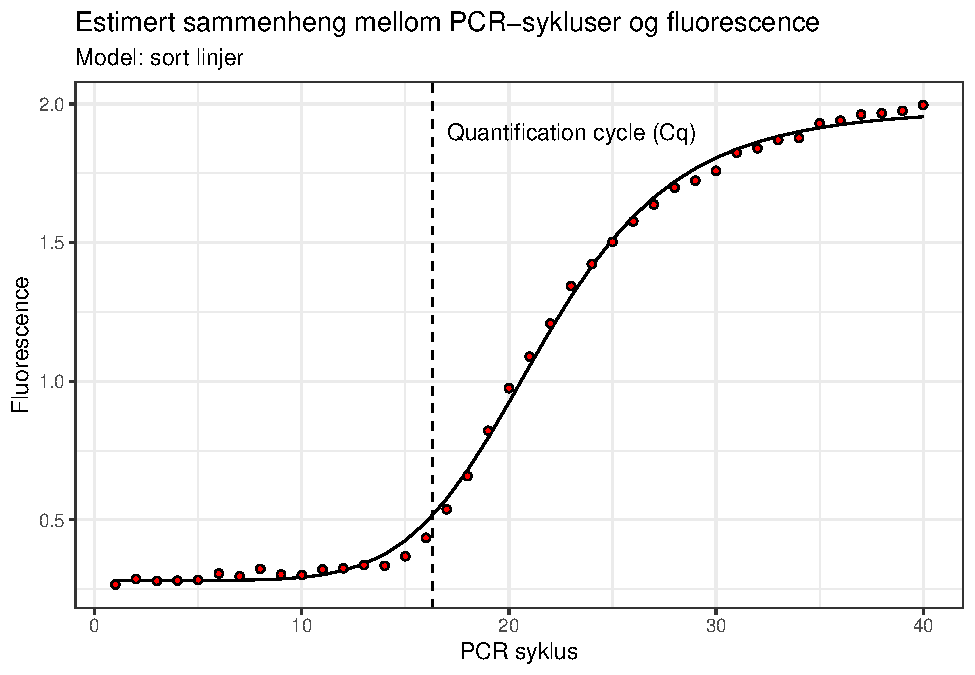
\includegraphics{_main_files/figure-latex/unnamed-chunk-3-1.pdf}

\hypertarget{resultater-1}{%
\section{Resultater}\label{resultater-1}}

Modellen viser sammenhengen mellom antall sykluser og fluorescence.
Flere PCR-sykluser gir flere kopier, og dermed også en økt konsentrasjon i prøven.
På denne måten kan vi bruke fluorescence til å si noe om hvor mange sykluser som må til for å oppnå en bestemt terskelverdi(Cq-verdi).
Med primerne vi benyttet i forsøket var det ønskelig med et sted mellom 10 og 40 sykluser for å sikre at vi oppnådde terskelverdien. Det ble derfor kjørt 40 sykluser.

\begin{Shaded}
\begin{Highlighting}[]
\CommentTok{\#hvordan mengden av kopiert RNA utvikler seg med antall PCR{-}sykluser/Cq verdier??}
\NormalTok{cyc.diff }\OtherTok{\textless{}{-}} \FloatTok{3.327}
\NormalTok{dat }\OtherTok{\textless{}{-}} \FunctionTok{data.frame}\NormalTok{(}\AttributeTok{concentration =} \FunctionTok{c}\NormalTok{(}\DecValTok{1}\NormalTok{, }\DecValTok{1}\SpecialCharTok{/}\DecValTok{10}\NormalTok{, }\DecValTok{1}\SpecialCharTok{/}\DecValTok{100}\NormalTok{, }\DecValTok{1}\SpecialCharTok{/}\DecValTok{1000}\NormalTok{, }\DecValTok{1}\SpecialCharTok{/}\DecValTok{10000}\NormalTok{, }\DecValTok{1}\SpecialCharTok{/}\DecValTok{100000}\NormalTok{), }
           \AttributeTok{cq =} \FunctionTok{c}\NormalTok{(}\DecValTok{15}\NormalTok{, }
                  \DecValTok{15} \SpecialCharTok{+}\NormalTok{ cyc.diff,}
                  \DecValTok{15} \SpecialCharTok{+}\NormalTok{ cyc.diff}\SpecialCharTok{*}\DecValTok{2}\NormalTok{, }
                  \DecValTok{15} \SpecialCharTok{+}\NormalTok{ cyc.diff}\SpecialCharTok{*}\DecValTok{3}\NormalTok{, }
                  \DecValTok{15} \SpecialCharTok{+}\NormalTok{ cyc.diff}\SpecialCharTok{*}\DecValTok{4}\NormalTok{, }
                  \DecValTok{15} \SpecialCharTok{+}\NormalTok{ cyc.diff}\SpecialCharTok{*}\DecValTok{5}\NormalTok{)) }
\NormalTok{slope }\OtherTok{\textless{}{-}} \FunctionTok{coef}\NormalTok{(}\FunctionTok{lm}\NormalTok{(cq }\SpecialCharTok{\textasciitilde{}} \FunctionTok{log10}\NormalTok{(concentration), }\AttributeTok{data =}\NormalTok{ dat))[}\DecValTok{2}\NormalTok{]}
\NormalTok{dat }\SpecialCharTok{\%\textgreater{}\%}
  \FunctionTok{ggplot}\NormalTok{(}\FunctionTok{aes}\NormalTok{(cq, }\FunctionTok{log10}\NormalTok{(concentration)))  }\SpecialCharTok{+} 
  \FunctionTok{geom\_point}\NormalTok{() }\SpecialCharTok{+} \FunctionTok{geom\_smooth}\NormalTok{(}\AttributeTok{method =} \StringTok{"lm"}\NormalTok{) }\SpecialCharTok{+} 
  \FunctionTok{theme\_bw}\NormalTok{() }\SpecialCharTok{+} 
  \FunctionTok{annotate}\NormalTok{(}\StringTok{"text"}\NormalTok{, }\AttributeTok{x =} \DecValTok{15}\NormalTok{, }\AttributeTok{y =} \SpecialCharTok{{-}}\DecValTok{3}\NormalTok{, }\AttributeTok{hjust =} \DecValTok{0}\NormalTok{, }\AttributeTok{label =} \StringTok{"Efficiency factor \textasciitilde{} 2}\SpecialCharTok{\textbackslash{}n}\StringTok{ when slope \textasciitilde{} 3.3"}\NormalTok{)}
\end{Highlighting}
\end{Shaded}

\begin{verbatim}
## `geom_smooth()` using formula 'y ~ x'
\end{verbatim}

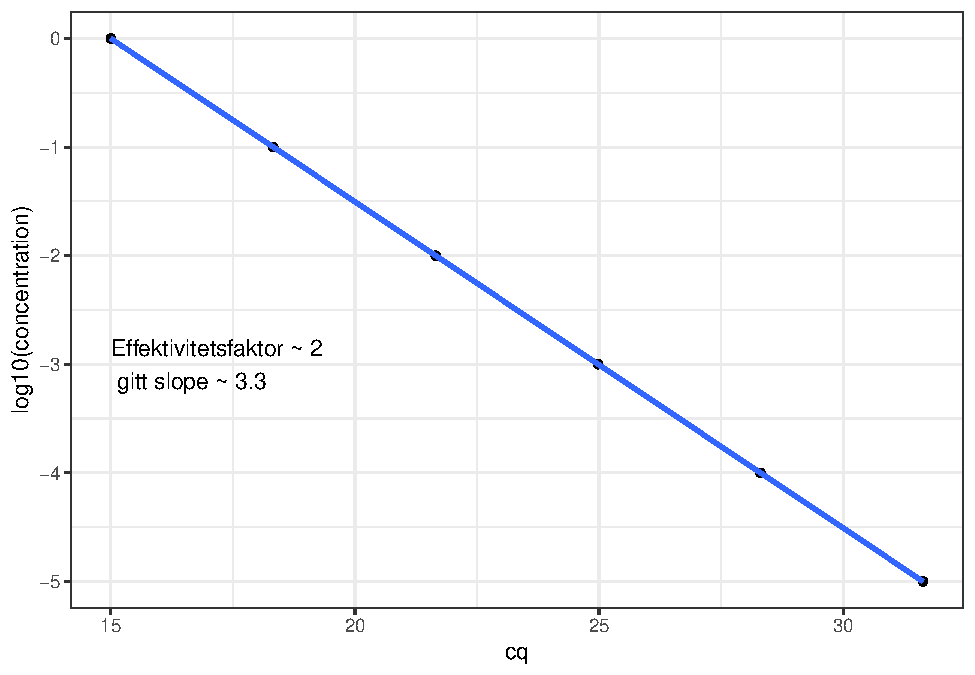
\includegraphics{_main_files/figure-latex/unnamed-chunk-4-1.pdf}

\begin{verbatim}
## `geom_smooth()` using formula 'y ~ x'
\end{verbatim}

\begin{figure}
\centering
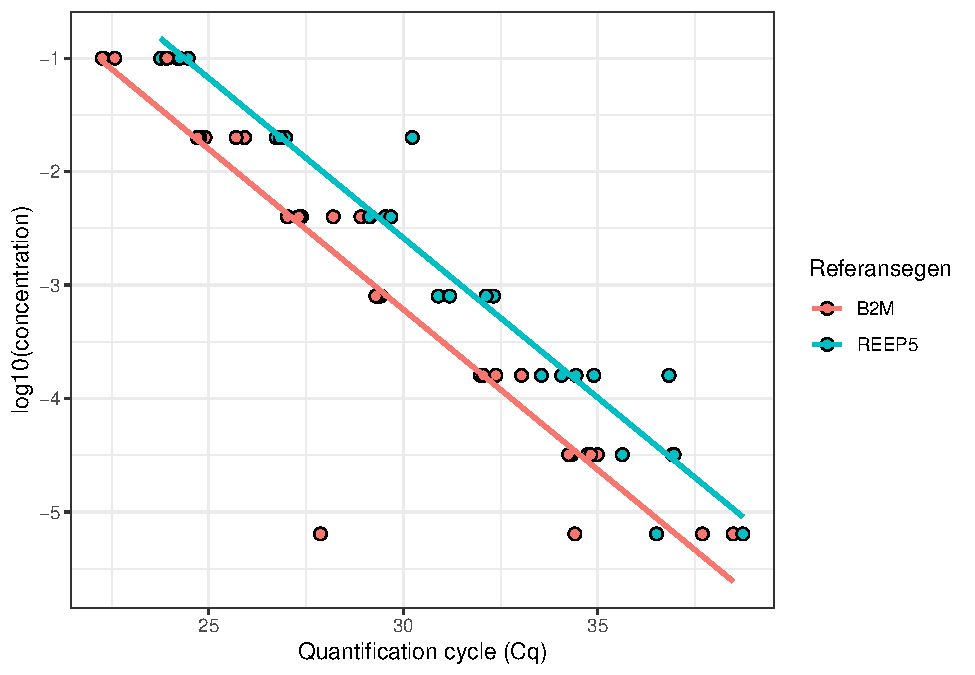
\includegraphics{_main_files/figure-latex/unnamed-chunk-5-1.pdf}
\caption{\label{fig:unnamed-chunk-5}Efficiency calculations made from serial dilution of cDNA}
\end{figure}

\begin{Shaded}
\begin{Highlighting}[]
 \CommentTok{\# Create models and extract the second coefficient from each model (the slope)}
\NormalTok{b2m\_slope }\OtherTok{\textless{}{-}} \FunctionTok{coef}\NormalTok{(}\FunctionTok{lm}\NormalTok{(cq }\SpecialCharTok{\textasciitilde{}} \FunctionTok{log10}\NormalTok{(concentration), }\AttributeTok{data =} \FunctionTok{filter}\NormalTok{(efficiency\_est\_data, target }\SpecialCharTok{==} \StringTok{"B2M"}\NormalTok{)))[}\DecValTok{2}\NormalTok{]}
\NormalTok{reep5\_slope }\OtherTok{\textless{}{-}} \FunctionTok{coef}\NormalTok{(}\FunctionTok{lm}\NormalTok{(cq }\SpecialCharTok{\textasciitilde{}} \FunctionTok{log10}\NormalTok{(concentration), }\AttributeTok{data =} \FunctionTok{filter}\NormalTok{(efficiency\_est\_data, target }\SpecialCharTok{==} \StringTok{"REEP5"}\NormalTok{)))[}\DecValTok{2}\NormalTok{]}
\CommentTok{\# Calculate and store the data in a data frame}
\NormalTok{efficiency\_estimates }\OtherTok{\textless{}{-}} \FunctionTok{data.frame}\NormalTok{(}\AttributeTok{target =} \FunctionTok{c}\NormalTok{(}\StringTok{"B2M"}\NormalTok{, }\StringTok{"REEP5"}\NormalTok{), }
           \AttributeTok{Efficiency =} \FunctionTok{c}\NormalTok{(}\DecValTok{10}\SpecialCharTok{\^{}{-}}\NormalTok{(}\DecValTok{1}\SpecialCharTok{/}\NormalTok{b2m\_slope), }
                          \DecValTok{10}\SpecialCharTok{\^{}{-}}\NormalTok{(}\DecValTok{1}\SpecialCharTok{/}\NormalTok{reep5\_slope)))}
\end{Highlighting}
\end{Shaded}

\begin{Shaded}
\begin{Highlighting}[]
\DocumentationTok{\#\# Estimerte cq verdier? }
\FunctionTok{library}\NormalTok{(flextable)}
\end{Highlighting}
\end{Shaded}

\begin{verbatim}
## 
## Attaching package: 'flextable'
\end{verbatim}

\begin{verbatim}
## The following object is masked from 'package:purrr':
## 
##     compose
\end{verbatim}

\begin{Shaded}
\begin{Highlighting}[]
\NormalTok{fc\_g1 }\OtherTok{\textless{}{-}}\NormalTok{ results\_group1 }\SpecialCharTok{\%\textgreater{}\%}
  \FunctionTok{separate}\NormalTok{(ID, }\AttributeTok{into =} \FunctionTok{c}\NormalTok{(}\StringTok{"well"}\NormalTok{, }\StringTok{"sample"}\NormalTok{, }\StringTok{"subsample"}\NormalTok{, }\StringTok{"time"}\NormalTok{, }\StringTok{"target"}\NormalTok{)) }\SpecialCharTok{\%\textgreater{}\%}
\NormalTok{  dplyr}\SpecialCharTok{::}\FunctionTok{select}\NormalTok{(well}\SpecialCharTok{:}\NormalTok{target, }\AttributeTok{cq =}\NormalTok{ cpD2) }\SpecialCharTok{\%\textgreater{}\%}
  \FunctionTok{filter}\NormalTok{(sample }\SpecialCharTok{\%in\%} \FunctionTok{c}\NormalTok{(}\StringTok{"FP1"}\NormalTok{, }\StringTok{"FP2"}\NormalTok{, }\StringTok{"FP3"}\NormalTok{)) }\SpecialCharTok{\%\textgreater{}\%}
\NormalTok{  dplyr}\SpecialCharTok{::}\FunctionTok{select}\NormalTok{(sample, time, target, cq) }\SpecialCharTok{\%\textgreater{}\%}
  \FunctionTok{mutate}\NormalTok{(}\AttributeTok{target =} \FunctionTok{toupper}\NormalTok{(target), }
         \AttributeTok{target =} \FunctionTok{gsub}\NormalTok{(}\StringTok{"RRNA475"}\NormalTok{, }\StringTok{"RRNA47S"}\NormalTok{, target)) }\SpecialCharTok{\%\textgreater{}\%}
  \FunctionTok{group\_by}\NormalTok{(sample)}\SpecialCharTok{\%\textgreater{}\%}
  \FunctionTok{pivot\_wider}\NormalTok{(}\AttributeTok{names\_from =}\NormalTok{ target, }\AttributeTok{values\_from =}\NormalTok{ cq) }\SpecialCharTok{\%\textgreater{}\%}
  \FunctionTok{arrange}\NormalTok{(time) }\SpecialCharTok{\%\textgreater{}\%}
   \FunctionTok{flextable}\NormalTok{() }\SpecialCharTok{\%\textgreater{}\%}
  \FunctionTok{print}\NormalTok{()}
\end{Highlighting}
\end{Shaded}

\begin{verbatim}
## Warning: Expected 5 pieces. Additional pieces discarded in 70 rows [1, 2, 3, 4,
## 5, 6, 7, 8, 9, 10, 11, 12, 13, 14, 15, 16, 17, 18, 19, 20, ...].
\end{verbatim}

\begin{verbatim}
## a flextable object.
## col_keys: `sample`, `time`, `MYHC1`, `MYHC2A`, `MYHC2X`, `RRNA47S`, `CHMP2A`, `REEP5`, `B2M` 
## header has 1 row(s) 
## body has 6 row(s) 
## original dataset sample: 
##   sample time MYHC1 MYHC2A MYHC2X RRNA47S CHMP2A REEP5   B2M
## 1    FP1   w0 19.53  20.03  22.87   24.88  26.68 26.68 23.79
## 2    FP2   w0 19.70  20.04  29.80   27.54  26.78 26.59 25.22
## 3    FP3   w0 20.33  18.25  22.87   25.27  25.97 26.55 24.53
## 4    FP1   w2 19.96  17.59  26.01   32.36  26.73 26.87 24.01
## 5    FP2   w2 20.20  14.64  26.23   27.00  26.45 26.40 24.56
\end{verbatim}

\hypertarget{diskusjon-1}{%
\section{Diskusjon}\label{diskusjon-1}}

Cq-verdien sier noe om hvor mange PCR-sykluser som trengs for å detektere ulike targets.En høyere Cq-verdi indikerer altså at mengden RNA må dobles flere ganger for å detektere en terskelverdi av target. En lavere Cq-verdi indikerer at terskelverdien oppnås ved færre PCR-sykluser, altså at konsentrasjonen av target er høyere. En lavere Cq-verdi ved uke 2, sammenlignet med uke 0(baseline) som i forsøket, indikerer høyere konsentrasjon ved uke 2 enn ved uke 0. (Dermed en effekt av intervensjonen, avhengig av funksjonen til target - gen).

\hypertarget{vitenskapsteori}{%
\chapter{Vitenskapsteori}\label{vitenskapsteori}}

Placeholder

\hypertarget{falsifikasjonisme}{%
\section{1. Falsifikasjonisme}\label{falsifikasjonisme}}

\hypertarget{hd-metoden-og-abduksjonbayesisme}{%
\section{2. HD-metoden og abduksjon/Bayesisme}\label{hd-metoden-og-abduksjonbayesisme}}

\hypertarget{replikasjonskrisen}{%
\section{3. Replikasjonskrisen}\label{replikasjonskrisen}}

\hypertarget{studiedesign}{%
\chapter{Studiedesign}\label{studiedesign}}

Placeholder

\hypertarget{introduksjon-1}{%
\section{Introduksjon}\label{introduksjon-1}}

\hypertarget{metode-2}{%
\section{Metode}\label{metode-2}}

\hypertarget{resultat}{%
\section{Resultat}\label{resultat}}

\hypertarget{videre-forskning}{%
\section{Videre forskning}\label{videre-forskning}}

\hypertarget{vs-3-sett}{%
\chapter{1 vs 3 sett}\label{vs-3-sett}}

Placeholder

\hypertarget{introduksjon-2}{%
\section{Introduksjon}\label{introduksjon-2}}

\hypertarget{metode-3}{%
\section{Metode}\label{metode-3}}

\hypertarget{etikk}{%
\subsection{Etikk}\label{etikk}}

\hypertarget{deltagere}{%
\subsection{Deltagere}\label{deltagere}}

\hypertarget{trening}{%
\subsection{Trening}\label{trening}}

\hypertarget{testing}{%
\subsection{Testing}\label{testing}}

\hypertarget{styrketester}{%
\subsubsection{Styrketester}\label{styrketester}}

\hypertarget{testing-av-muskelmasse}{%
\subsubsection{Testing av Muskelmasse}\label{testing-av-muskelmasse}}

\hypertarget{statestikk}{%
\subsection{Statestikk}\label{statestikk}}

\hypertarget{resultat-1}{%
\section{Resultat}\label{resultat-1}}

\hypertarget{muskelmasse}{%
\subsection{Muskelmasse}\label{muskelmasse}}

\hypertarget{muskelstyrke}{%
\subsection{Muskelstyrke}\label{muskelstyrke}}

\hypertarget{diskusjon-2}{%
\section{Diskusjon}\label{diskusjon-2}}

\hypertarget{treningsanbefaling}{%
\subsection{Treningsanbefaling}\label{treningsanbefaling}}

\hypertarget{konklusjon}{%
\subsection{Konklusjon}\label{konklusjon}}

  \bibliography{book.bib}

\end{document}
